\section{Examples, reproducibility and verification status}
\label{app:verification}

\subsection{The first two zeta ordinates as an illustration}

For the first two positive zeta ordinates, numerical approximations give
\[
 \gamma_1\approx14.13472514173469,\qquad
 \gamma_2\approx21.02203963877155,\qquad
 \gamma_2/\gamma_1\approx1.48726200389289.
\]
These values are used only for illustration. The exact theorem applies
to their exact values. As the ratio is in the first band, the least
logarithmic width for a positive average cancelling both is
\[
 b=\frac{4\pi}{\gamma_1+\gamma_2}
   \approx0.3574381969676284,
 \qquad e^b\approx1.4296622062580134.
\]
Thus three positive weights at the multiplicative scales
$1,e^{b/2},e^b$ suffice, and no positive measure of smaller logarithmic
support diameter can cancel these two exact frequencies. Tilting by the
common real part $1/2$ gives the following numerical weights.

\begin{center}
\begin{tabular}{@{}rr@{}}
\toprule
Logarithmic shift & Positive weight\\
\midrule
$0$ & $0.300320635800919$\\
$0.178719098483814$ & $0.448508964657668$\\
$0.357438196967628$ & $0.251170399541413$\\
\bottomrule
\end{tabular}
\end{center}

The script uses 85-digit arithmetic and computes the residual of both
exponential moments. The displayed decimal weights are rounded and do
not cancel exactly. Exact cancellation refers to the defining formulas
with the exact ordinates. These computations do not certify numerical
zero enclosures or zero simplicity.

\begin{figure}[p]
 \centering
 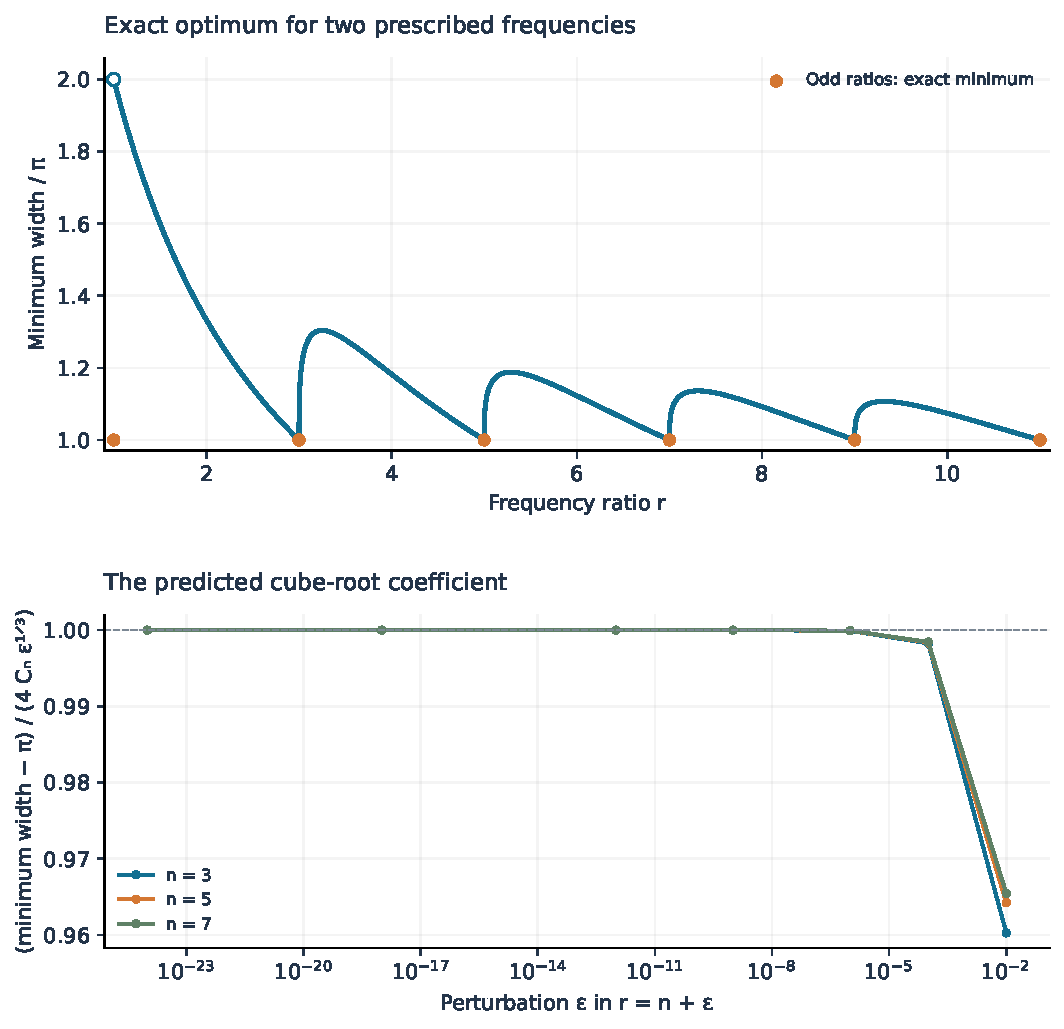
\includegraphics[width=\textwidth]{figures/filter_phase_diagram.pdf}
 \caption{The proven optimum and its resonance asymptotic, illustrated
 numerically. The values at odd ratios are exactly $\pi$. At ratio $1$
 the two constraints coincide; its value is $\pi$, although the
 right-hand limit is $2\pi$. In the second panel, the normalized excess
 tends to one as predicted by Theorem~\ref{filt:cusp}. This figure is
 generated from the supplied script, not from a source image.}
 \label{fig:phase}
\end{figure}

\subsection{What the executable checks establish}

The proof is analytic. The accompanying computations are consistency
checks aimed at arithmetic errors, incorrect signs and incorrect leading
constants. The Python files state their own scope.

\begin{center}
\small
\begin{tabular}{@{}p{.27\linewidth}p{.63\linewidth}@{}}
\toprule
Artifact & Result and limitation\\
\midrule
\texttt{filter\_checks.py} & 19 frequency-ratio examples satisfy the two
moments to better than $2\cdot10^{-85}$ in the recorded run. The
nonnegative certificate was also sampled. Numerical sampling is not
a proof of positivity.\\[4pt]
Linear programs & Ten ratio cases were discretized on
4001 nodes. The solver returned no feasible solution below the optimum
and a feasible solution above it. Discretized feasibility is only a
cross-check.\\[4pt]
\texttt{cusp.csv} & 28 high-precision cases for odd ratios
$3,5,7,11$ check the cube-root coefficient and the limiting inner mass
$2/3$.\\[4pt]
\texttt{real\_weight\_checks.py} & Exact arithmetic in
$\mathbb Q(\sqrt2)$ verifies 65 telescoping identities and recovers
13 target multiplicities, including zeros, asymmetric pairs and repeated
atoms. One fixture forces three rejected stopping points.\\[4pt]
Two-center obstruction & 364 exact queries check the two periodic
counterexample spectra, and an irrational third center distinguishes
them. The general proof is Proposition~\ref{rw:prop:reflection}.\\
\bottomrule
\end{tabular}
\end{center}

The results are preserved in machine-readable JSON and CSV. They are
reproduced by running, from the archive directory,
\begin{verbatim}
python3 scripts/filter_checks.py
python3 scripts/real_weight_checks.py \
  --output results/real_weight_checks.json
latexmk -pdf -interaction=nonstopmode -halt-on-error report.tex
\end{verbatim}
The exact reconstruction script needs only the Python standard library.
The filter script additionally needs \texttt{mpmath}, \texttt{numpy},
\texttt{scipy} and \texttt{matplotlib}. The PDF is compiled from the
included LaTeX source and bibliography. No repository access is needed
to reproduce these examples or rebuild this note.

\subsection{Proof review and a route to formal verification}

The source analysis and both new proofs were checked in separate review
passes during this AI-assisted research session. This is not external
peer review. No substantive gap was identified in those passes. The
verification notes preserve the checked signs, conductor-uniform error
bound, infinite-sum argument, reflection scope and exact-oracle
qualification. The following are the main modules for a future Lean
formalization; they are a plan, not implemented declarations.

\begin{enumerate}
\item \emph{Positive arithmetic encoder.} Formalize the multiquadratic
separation lemma and its effective tail construction. Obtain the shifted
first-Riesz explicit formula uniformly in the conductor. Prove the
Fourier--Bohr autocorrelation identity for absolutely summable frequency
families, including collisions. Combine it with integer decoding and
the discrete reflection/Pell argument. Only the explicit-formula module
uses Dirichlet GRH.
\item \emph{Two-frequency optimum.} Formalize the derivative of
$s\cos(ru)/\cos u$, its last positive lobe, and the unique outer root.
Use the nonnegative certificate to restrict the support of every
admissible measure. Finite-dimensional linear algebra gives unique
weights without an assumed symmetry. Formalize the scaled analytic
implicit-function argument to obtain the cube-root law with its
remainder. The shortening proof uses a perturbed certificate and an
explicit competing measure.
\end{enumerate}

The new results here have complete ordinary mathematical proofs, but no
claim is made that they have been accepted by Lean. The upstream GRH
formalization remains an external, separately checked input.

\subsection{Further questions suggested by the two results}

The real encoder deliberately trades numerical conditioning for exact
identifiability. A useful next question is whether a finite family of
bounded-conductor characters admits one positive real weight with
quantitative finite-time reconstruction guarantees under explicit
separation assumptions, or with a weaker metric that tolerates clusters.
The present proof supplies the exact target and separates reflection
ambiguity from coefficient decoding.

For positive cancellation, three arbitrary noncommensurate frequencies
produce a higher-dimensional moment curve. Determining its minimum
width, all support transitions and the possible fractional powers at
resonances would extend the two-frequency theorem. Requiring vanishing
jets at both frequencies is another problem: the simple cancellation
proved here does not automatically supply derivative cancellation.
